\documentclass[journal]{vgtc}                % final (journal style)
%\documentclass[review,journal]{vgtc}         % review (journal style)
%\documentclass[widereview]{vgtc}             % wide-spaced review
%\documentclass[preprint,journal]{vgtc}       % preprint (journal style)
%\documentclass[electronic,journal]{vgtc}     % electronic version, journal

%% Uncomment one of the lines above depending on where your paper is
%% in the conference process. ``review'' and ``widereview'' are for review
%% submission, ``preprint'' is for pre-publication, and the final version
%% doesn't use a specific qualifier. Further, ``electronic'' includes
%% hyperreferences for more convenient online viewing.

%% Please use one of the ``review'' options in combination with the
%% assigned online id (see below) ONLY if your paper uses a double blind
%% review process. Some conferences, like IEEE Vis and InfoVis, have NOT
%% in the past.

%% Please note that the use of figures other than the optional teaser is not permitted on the first page
%% of the journal version.  Figures should begin on the second page and be
%% in CMYK or Grey scale format, otherwise, colour shifting may occur
%% during the printing process.  Papers submitted with figures other than the optional teaser on the
%% first page will be refused.

%% These three lines bring in essential packages: ``mathptmx'' for Type 1
%% typefaces, ``graphicx'' for inclusion of EPS figures. and ``times''
%% for proper handling of the times font family.

\usepackage{mathptmx}
\usepackage{graphicx}
\usepackage{times}



%% We encourage the use of mathptmx for consistent usage of times font
%% throughout the proceedings. However, if you encounter conflicts
%% with other math-related packages, you may want to disable it.

%% This turns references into clickable hyperlinks.
\usepackage[bookmarks,backref=true,linkcolor=black]{hyperref} %,colorlinks
\hypersetup{
  pdfauthor = {},
  pdftitle = {},
  pdfsubject = {},
  pdfkeywords = {},
  colorlinks=true,
  linkcolor= black,
  citecolor= black,
  pageanchor=true,
  urlcolor = black,
  plainpages = false,
  linktocpage
}
\usepackage[hyphenbreaks]{breakurl}

%% If you are submitting a paper to a conference for review with a double
%% blind reviewing process, please replace the value ``0'' below with your
%% OnlineID. Otherwise, you may safely leave it at ``0''.
\onlineid{0}

%% declare the category of your paper, only shown in review mode


%% allow for this line if you want the electronic option to work properly


%% In preprint mode you may define your own headline.
%\preprinttext{To appear in an IEEE VGTC sponsored conference.}

%% Paper title.

\title{Visual Analytics on World University Rankings }
%\subtitle{Visual Analytics project, A.Y. 2017/2018}

%% This is how authors are specified in the journal style

%% indicate IEEE Member or Student Member in form indicated below
\author{Valerio Evangelisti}


%other entries to be set up for journal
%\shortauthortitle{Firstauthor \MakeLowercase{\textit{et al.}}: Paper Title}

%% Abstract section.
\abstract{
The project here described was developed to put into practice all teachings
of the Visual Analytics course. It concerns the visualization of world university 
rankings to let the user have a clearer idea about the world university context.
All data are represented using well-known views to keep the interface as
simple as possible to interact with.


} % end of abstract

%% Keywords that describe your work. Will show as 'Index Terms' in journal
%% please capitalize first letter and insert punctuation after last keyword


%% ACM Computing Classification System (CCS).
%% See <http://www.acm.org/class/1998/> for details.
%% The ``\CCScat'' command takes four arguments.


%% Uncomment below to include a teaser figure.
  \teaser{
 \centering
 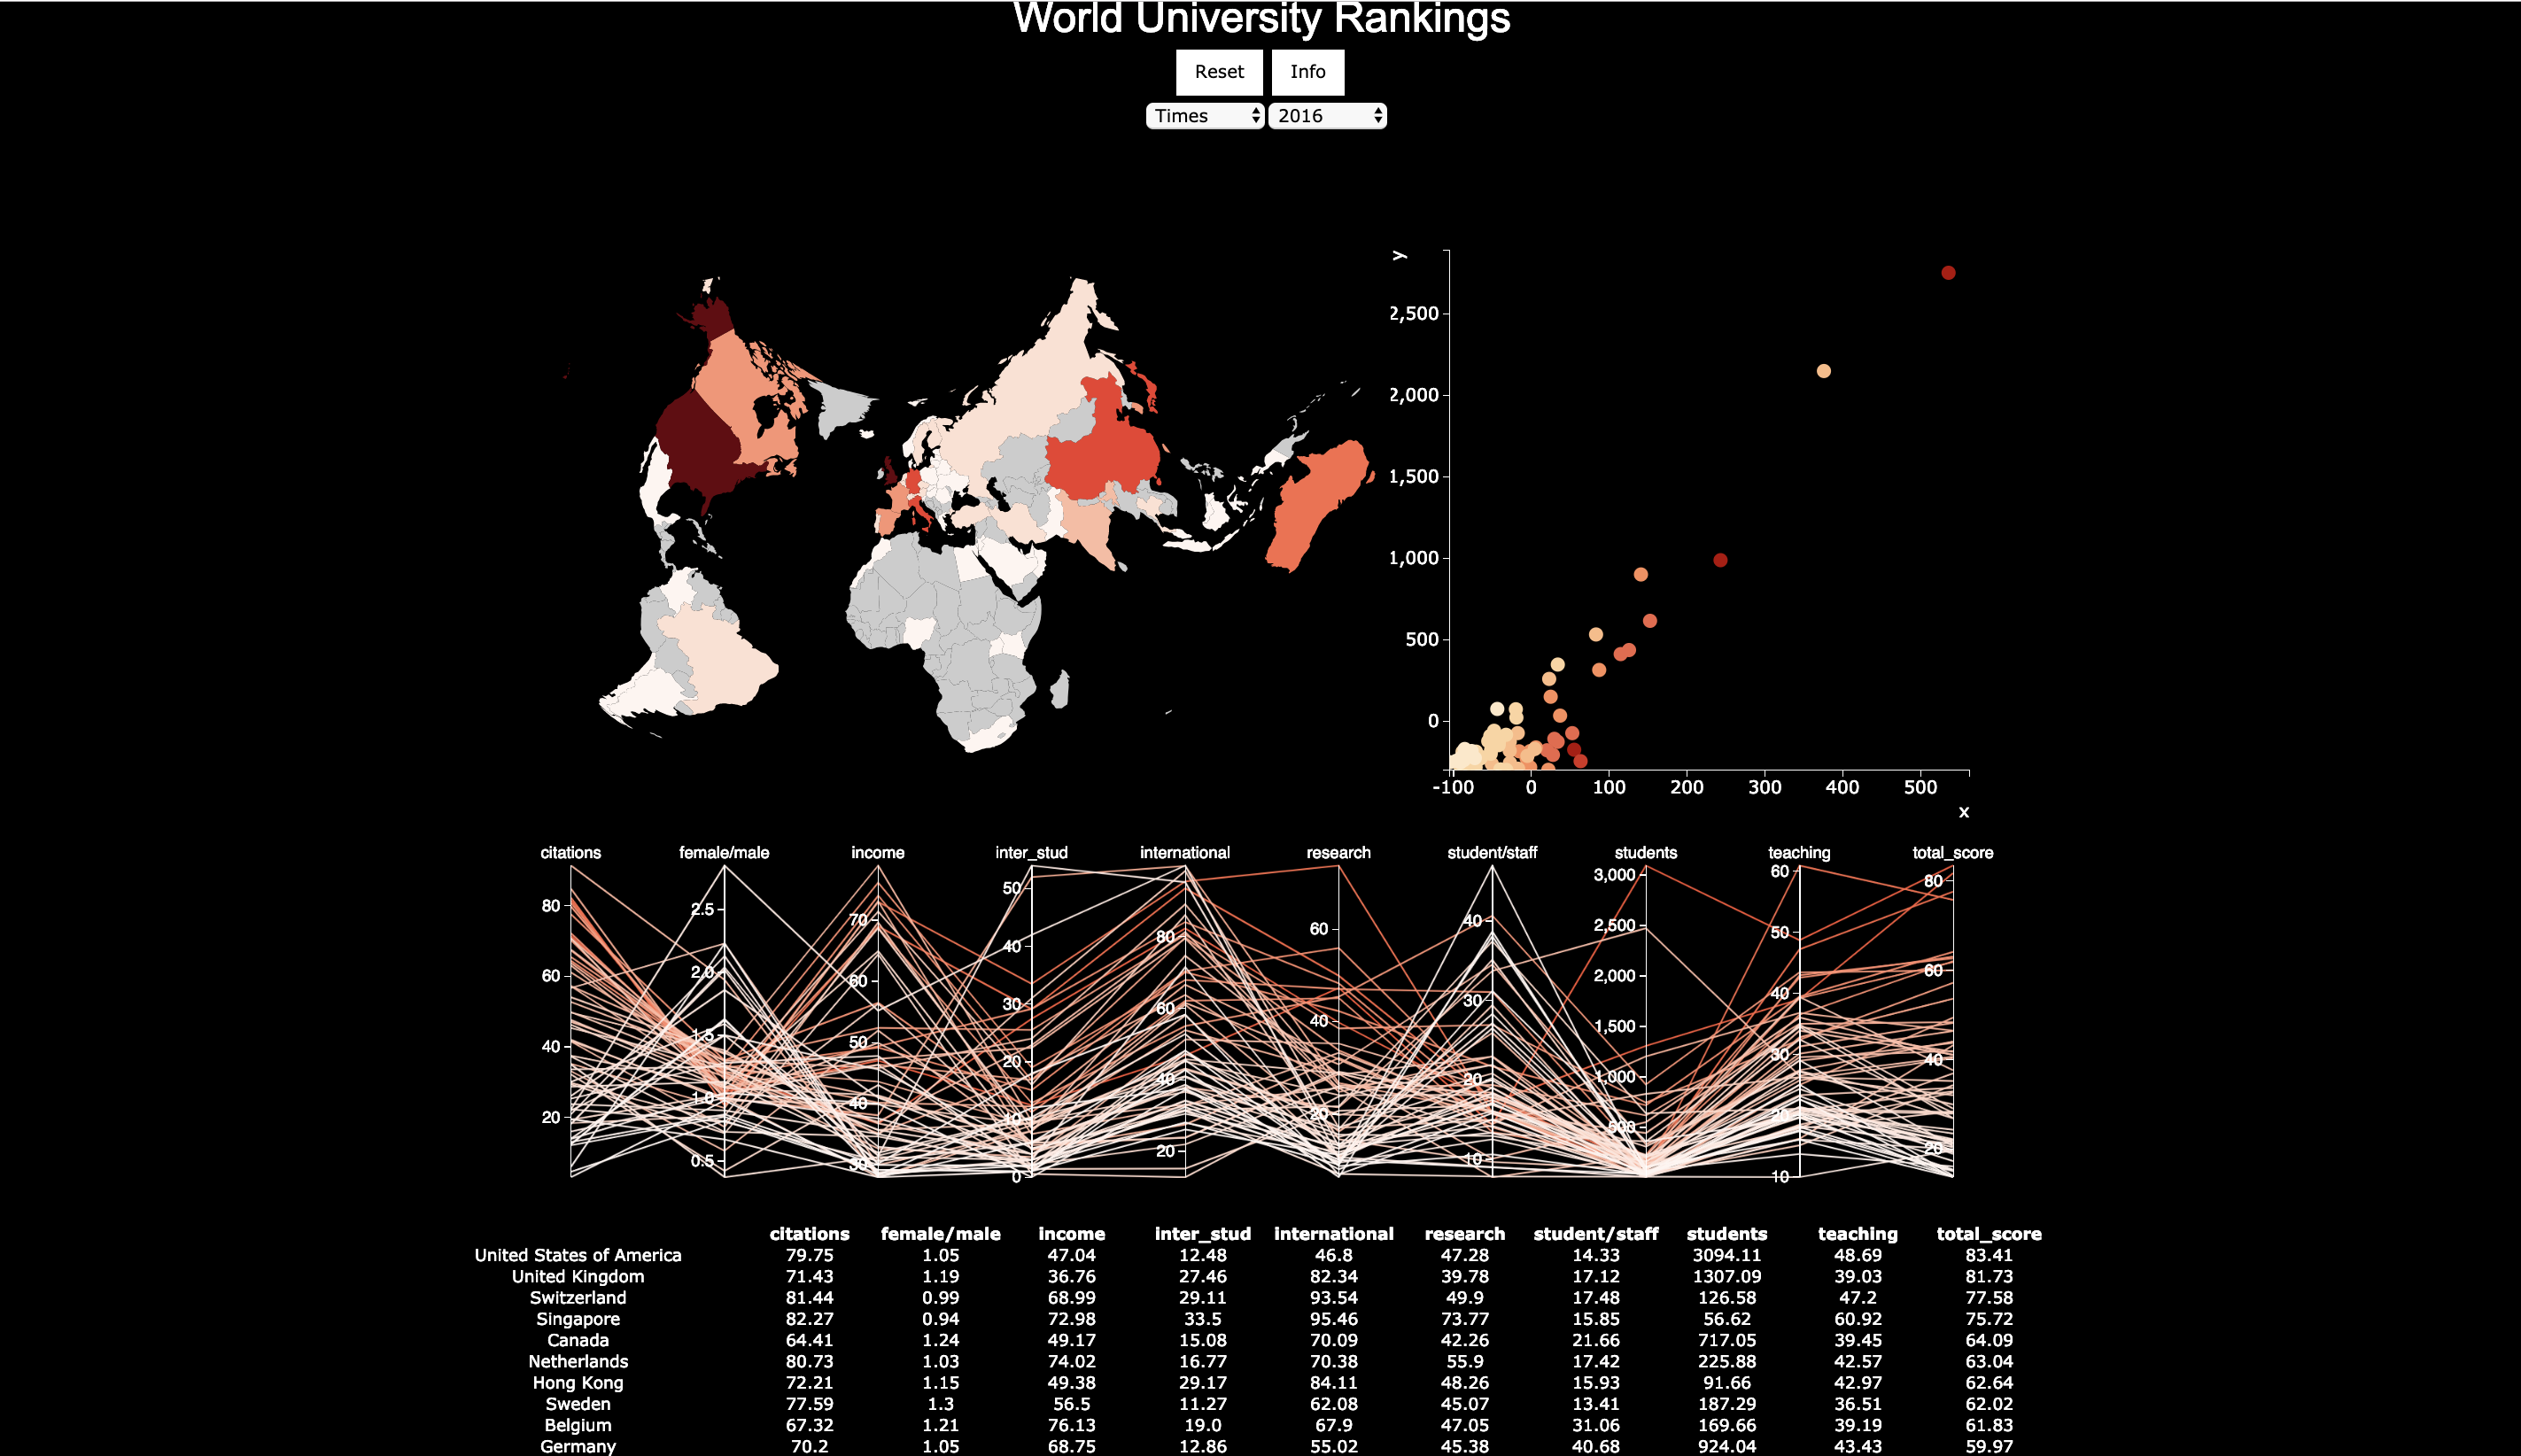
\includegraphics[width=16cm]{views}
  \caption{Sceenshot of the entire interface.}
  }

%% Uncomment below to disable the manuscript note
\renewcommand{\manuscriptnotetxt}{}

%% Copyright space is enabled by default as required by guidelines.
%% It is disabled by the 'review' option or via the following command:
 \nocopyrightspace

%%%%%%%%%%%%%%%%%%%%%%%%%%%%%%%%%%%%%%%%%%%%%%%%%%%%%%%%%%%%%%%%
%%%%%%%%%%%%%%%%%%%%%% START OF THE PAPER %%%%%%%%%%%%%%%%%%%%%%
%%%%%%%%%%%%%%%%%%%%%%%%%%%%%%%%%%%%%%%%%%%%%%%%%%%%%%%%%%%%%%%%%

\begin{document}

%% The ``\maketitle'' command must be the first command after the
%% ``\begin{document}'' command. It prepares and prints the title block.

%% the only exception to this rule is the \firstsection command
\firstsection{Introduction}

\maketitle

%% \section{Introduction} %for journal use above \firstsection{..} instead

In a world where it's easier and easier to move across country, many students face the 
problem to find the right university to conclude their educational program.

I am thinking about the need for a student to have the most of the informations available in 
only one platform, so that it's easier to compare different countries and universities.

Three of the most famous rankings are taken in consideration in this program:
\begin{itemize}
\item Times: takes into consideration some aspects such as the mark for what regards citations, teaching, research, international and some ratio such as the female/male ratio and the student/staff ones.
\item Shanghai: take into consideration the rewards and citations of a university
\item Cwur: it's a world ranking based on the quality of some aspects such as faculty, education, employment and so on.
\end{itemize}


\section{Dataset}
The dataset used in this project is taken from Kaggle database , it contains about more than 10000 tuples, each with an average of 10 attributes.
Some tuples lack of some values and so they were all removed in order to have a completely useful dataset. A few attributes for each remaining tuple were also removed because they were of no interest for us. I get in this way a more manageable dataset thanks to a lower number of tuples (ca. 7000) and of attributes (ca. 10).

It's possible to notice that the dataset gives us data for different years
so that it's possible to visualise the improvement or not of some countries or universities in the last decade.
It's likely to be another important factor of choice.


\section{Visualization}
The visualization that I have developed is constituted by 4 views.

Some of them are coordinated each other, so clicking on an element of a
certain view, the event handler will highlight some elements in the
others and/or will show other information. 

The user can choose thanks to a select form which ranking and year he wants to see.

In details, the map lets select countries for which the user wants to know more,
the scatterplot is the representation of an MDS algorithm that visualise the 
distance between countries or universities.
At the bottom of the page I have a parallel line chart that plots the specific value,
this value are than classified below it in a ranking in which the precise value for each 
characteristic is expressed.

The interface was thought to fit in a FullHD (1920x1080) screen,
even if it works also if we resize the browser window (the minimum
resolution supported is 1440x1080).


\subsection{Map}


\begin{figure}[h]
  \centering
  \includegraphics[scale=0.30]{map}
  \caption{Map in which the nations are coloured considering the number of university inside the specific rank}
  \label{map}
\end{figure}


The map is the first element that allows the user to interact with the application.
On the basis of the user choice, nations are coloured darker and darker depending on 
the number of university of that nation present in the ranking.
Clicking on a nation lunches a new analytic that compute all the necessary data for the
selection.

\subsection{Scatterplot}
\begin{figure}[h]
 \centering
  \includegraphics[scale=0.30]{scatterplot}
  \caption{Scatterplot that represents the whole dataset. Each point is a nation/university and the colour of the point encodes the total score of each}
  \label{scatterplot}
\end{figure}
Each point in the scatterplot represents a nation or a university and the colour encodes the total score. I used two different colour scaling  \texttt{d3.scaleQuantize().range(d3.schemeOrRd[9])}\cite{d3:2018}  and  \texttt{d3.scaleQuantize().range(d3.schemeYlGn[9])}\cite{d3:2018}. The choice of which use depend on how many countries the user select. In case of single selection, the scatterplot will show the university of the corresponding nation whit the first colour scheme. Instead if the choice is of two nations, the scatter will plot the universities of both countries but with different colour to let the user distinguish better the differences.


Due to the high number of element of the dataset, it was mandatory to apply an algorithm that let visualise everything better. I decided to apply MDS \cite{sklearn:2018} . It computes the level of similarity of individual cases of a dataset, returning the result with the two coordinates x and y
A 2D scatterplot is the best way to graphically represent the relation between points and to spot possible clusters. In this case it helps the student to quickly see that most of the bad and good universities are grouped together in a particular area.

Each point has associated two event handlers. The first one allows to make visible a tooltip showing the name of the country/university just by mouseovering over it.
The second handler is associated to click events: by clicking on two different points on the scatterplot, it will show a popup table with the comparison of the two selected elements.

\subsection{Parallel Coordinates}
\begin{figure}[h]
  \centering
  \includegraphics[scale=0.20]{parallel}
  \caption{Parallel Coordinates that represents the whole dataset, one line for each country/university. The color again encodes the classification of the customer}
  \label{parallel}
\end{figure}

Parallel Coordinate view is one of the best way to represent data with more than two dimensions in a 2D space. 

Depending on which ranking is chosen by the user, the chart will have a different numbers of columns. Each line in the Parallel Coordinate chart represent one country/university.

Thanks to a brushing event handler it is possible to apply some filters to this chart, so that the user can visualise better what it's more important for him.
It is also possible change the position of the y-axis to let the user visualise the chart as he prefers.

This chart is strongly related to the table below it.

\subsection{Table}

\begin{figure}[h]
  \centering
  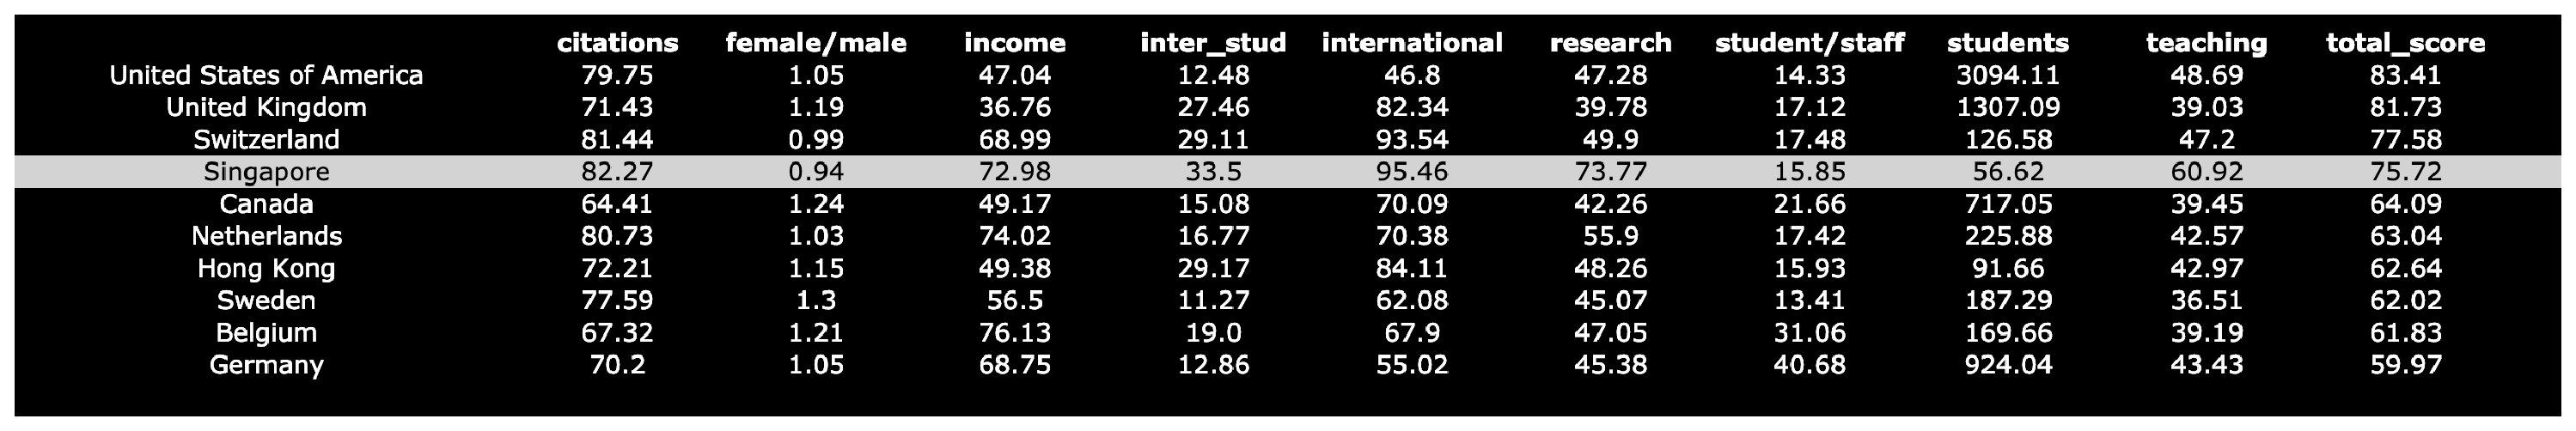
\includegraphics[scale=0.18]{table}
  \caption{Table in which are showed the 10 better countries/university in the selection}
  \label{Table}
\end{figure}

As said before, this table is strongly related to the Parallel Coordinate chart. This table will show the first ten element in the specific ranking or in the specific selection made by the user form the map or the Parallel chart. 

To let this table be more understandable and complete the integration with the above chart, a mouseover handler make not only the selected row to highlight (so that the user is not confused between all the numbers) but also highlight the corresponding line in the Parallel chart.

\begin{figure}[h]
  \centering
  \includegraphics[scale=0.18]{light}
  \caption{Table in which are showed the 10 better countries/university in the selection}
  \label{Table}
\end{figure}
\section{Analytics}

Since Javascript is not so fast handling large amount of data and it is not suitable doing intense computations, we needed to move the analytics part into a python program.

To do so, I set up a small web server using the python library \texttt{flask} that can communicate with the visualization.

The visualisation can be accessed after the server is started at the address \texttt{http://127.0.0.1:5000} (or \texttt{http://localhost:5000}). 

At the lunch of the serve it will execute the precompute.py file, in which are calculated all the years present in the rankings (so that is possible to have an updated program) and than compute the weighted average of all universities, grouped in countries, for the last year present and the MDS for those countries.

After the initialisation all the choice the user made are passed to the server with a   \texttt{getJson()} that, considering al the choices, call one of the three files: analytics.py, analytics1.py, analytics2.py.

The choice that triggers the  \texttt{getJson()} are: 
\begin{itemize}
\item Change of the ranking
\item Change of the year
\item Selection of one or more conuntry/ies: in this case there is the differentiation between the three analytics files.
At the beginning when no countries are selected it will calculate the national average from all the university for each country. If the user select one or two nations it will calculate the MDS for all the university of one or both countries and display il with all the other informations. If the selection is bigger than 2, the MDS is calculated between the weighted average result of the selected countries.
\end{itemize}

The result of those analytics are saved in two different csv files. 



\section{Conclusion}

In this work I wanted to help first of all students who need to search as much informations as possible in the clearest way possible. It's not absurd thinking about this project as a program useful to govern, administration or universities to have a worldwide knowledge about culture and how/where to improve to challenge the best ones.
This program has a fluid visualisation with no lags but need a little bit of time in the computation of new large amount of data, such as during the change of ranking or for particular countries cases.

\bibliographystyle{abbrv}
%%use following if all content of bibtex file should be shown
%\nocite{*}
\bibliography{template}
\end{document}
